\newpage
\chapter{MXP for High Performance Computing}

\section{VectorBlox MXP Matrix Processor}
VectorBlox MXP is a scalable supercomputer on FPGA. It is a SIMD accelerator, available as an IP core. MXP consist of the scratchpad memory which is its local memory and all vector operations are performed directly upon it which maximizes its performance. Unlike traditional processors which have address and data registers, there are no load-stores of vector data in MXP \cite{20}. The architecture of MXP is composed of DMA engine and vector engine. MXP soft-processor provides maximum improved performance because the DMA and vector engine can run at a frequency which is different from the host CPU frequency. DMA engine is used to transfer the data to the local scratchpad. Since MXP implements DMA to access the DDR memory directly, the cache-hierarchy is bypassed. Vector engine is composed of multiple parallel vector lanes, the number of which can be configured from 1 to 256 and 4KB of scratchpad is available for each vector lane. Each lane consists of 32-bit ALU and 4KB of scratchpad memory. The scratchpad and ALU can be divided to perform operations on 16-bits/halfword or 8-bits/byte of data. Thus, the architecture of the MXP soft processor during the byte (8-bits) and half-word (16-bits) level operation provides four and two times the performance respectively as compared to the performance obtained for word level operation. 

\begin{figure}
	\centering
	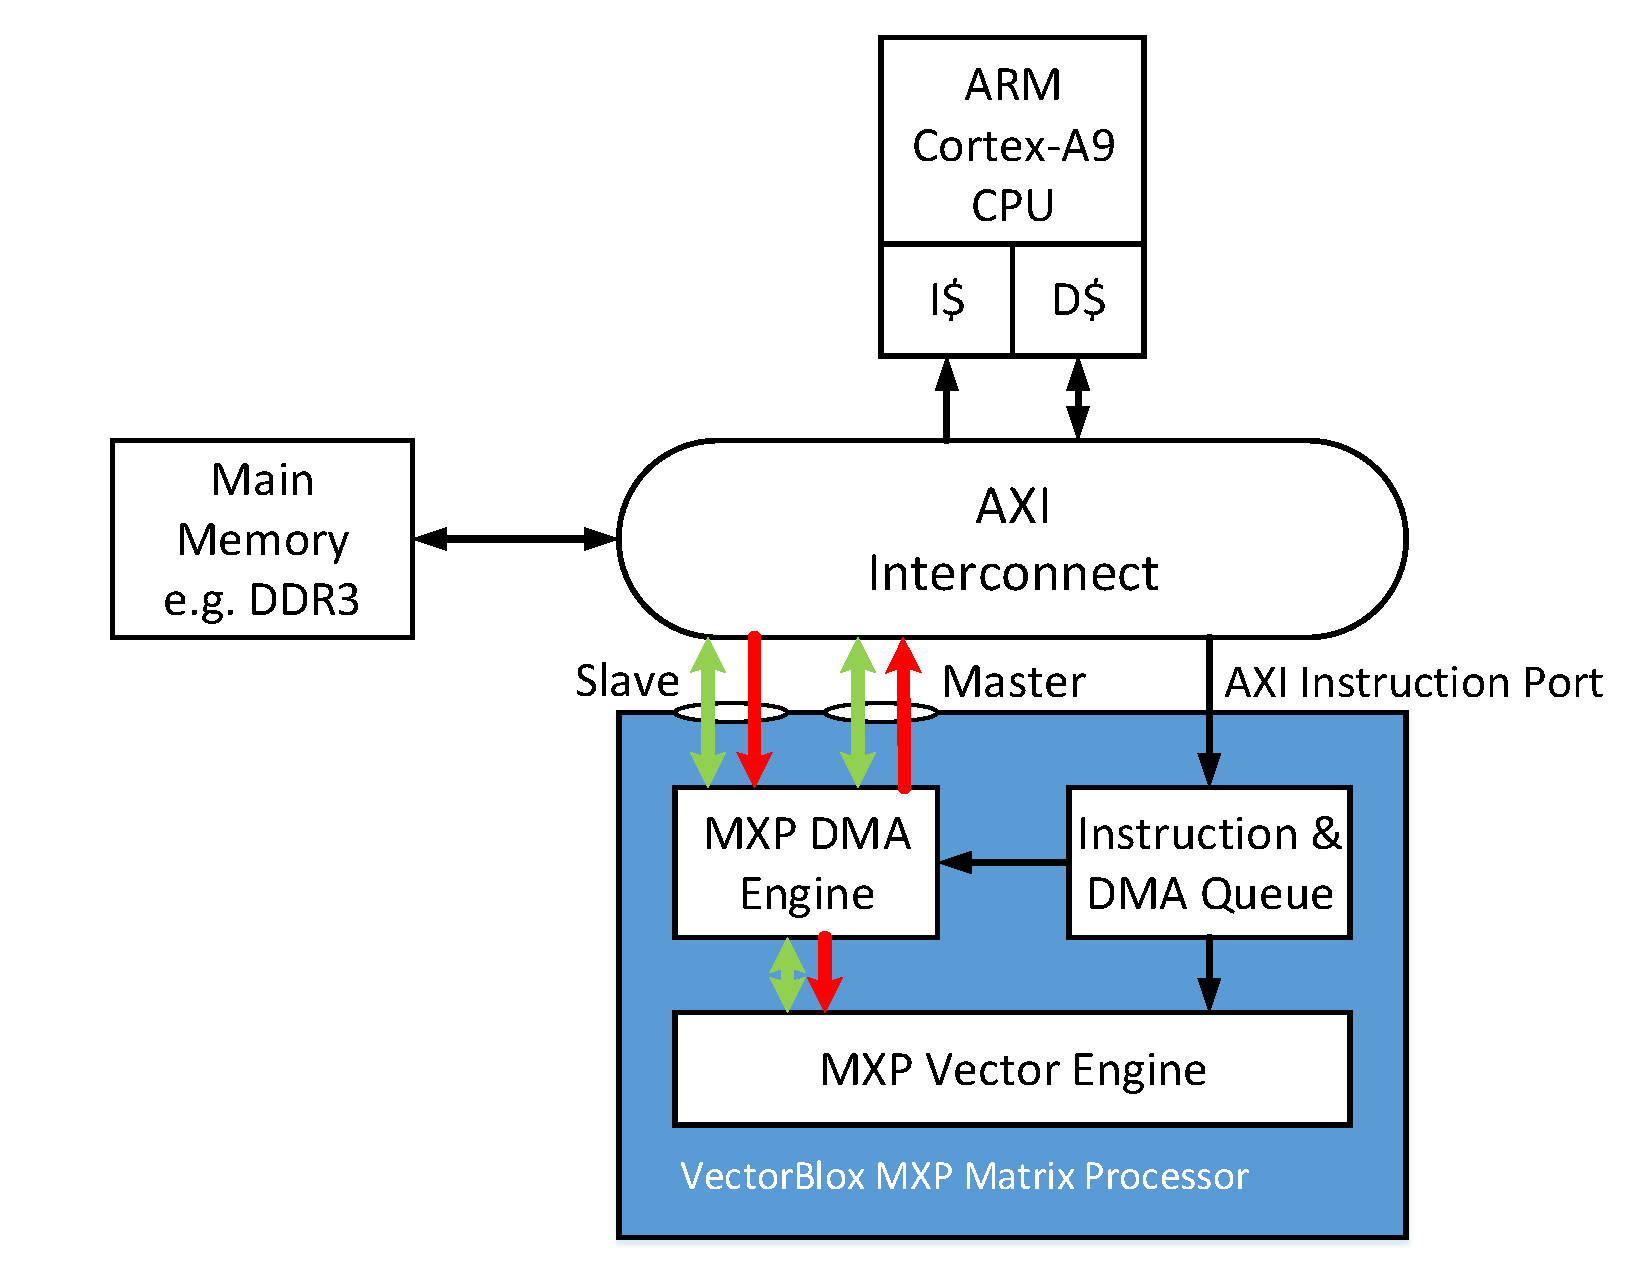
\includegraphics[width=0.9\textwidth]{images/mxp_diagram.pdf}
	\caption{Matrix Processor on ZedBoard\cite{20}}
	\label{zynq:mat}
\end{figure}

MXP vector processor is instantiated onto the programmable logic of the Zynq ZedBoard SoC as shown in Figure~\ref{zynq:mat}. The communication with ARM processor happens via general purpose ports whereas high performance ports are used for communication with the DDR memory. With 64 KB of scratchpad, we can put 32 16-bit lanes/ 16 32-bit lanes / 64 8-bit lanes. The instruction port uses a dedicated AXI slave interface connecting to master GP port on PS. The scratchpad also connects its slave interface to PS through one of the master GP ports. The DMA engine is connected to the DDR memory controller though AXI slave HP ports. Maximum frequency achievable for the 16-lane MXP soft processor is 110 MHz.

VectorBlox MXP can exploit the data parallelism in the computation by organizing the hardware into a tightly coupled array of the compute units that all execute the same instruction in the same cycle.

\subsection{Scratchpad}
MXP do not consist of any data or address registers. It performs all computations using scratchpad. This is used to maximize the performance as it prevents in performing the fetch and load. It does not require additional memory to hold the values.

The primary mechanism to transfer the data to the scratchpad is using the DMA (Direct Memory Access). Host processor can access the elements present in the scratchpad directly.

\subsection{Other Processor State}
MXP soft-processor consist of 32 bits control registers. First 16 registers are used for only hardware. Second group of control registers are software defined.

\subsection{Overlapping Communication with Computation}
Overlapping of the Communication with Computation is necessary to obtain maximum performance. Large set of data are processed usually by decomposing the computation into smaller blocks which further depends on the scratchpad size, and processing chunk of block simultaneously when other block is being transferred. Hence, the time required for transferring the data to the local scratchpad is hidden during the actual computation.   

\begin{figure}
	\centering
	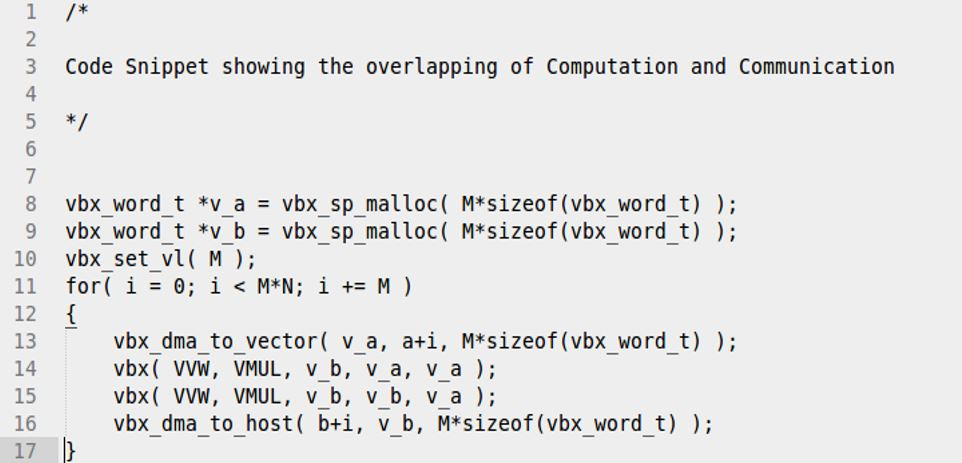
\includegraphics[width=0.9\textwidth]{images/c1.png}
	\caption{Overlapping of the Computation and Communication}
	\label{c1:mat}
\end{figure}

For example, consider the code in figure~\ref{c1:mat}, which calculates the cube of a and puts the result in variable b. It utilizes small blocks having size of M and the dataset being used is having a size of M*N.

For improved performance and efficiency, the code can be rewritten in such a way that the computation and communication can be overlapped. Double buffering is one of the methods through which you can achieve the overlapping of computation and communication. In this technique, one buffer holds the current processing data while the other buffer job is to transfer data in and out of the local scratchpad.

\begin{figure}
	\centering
	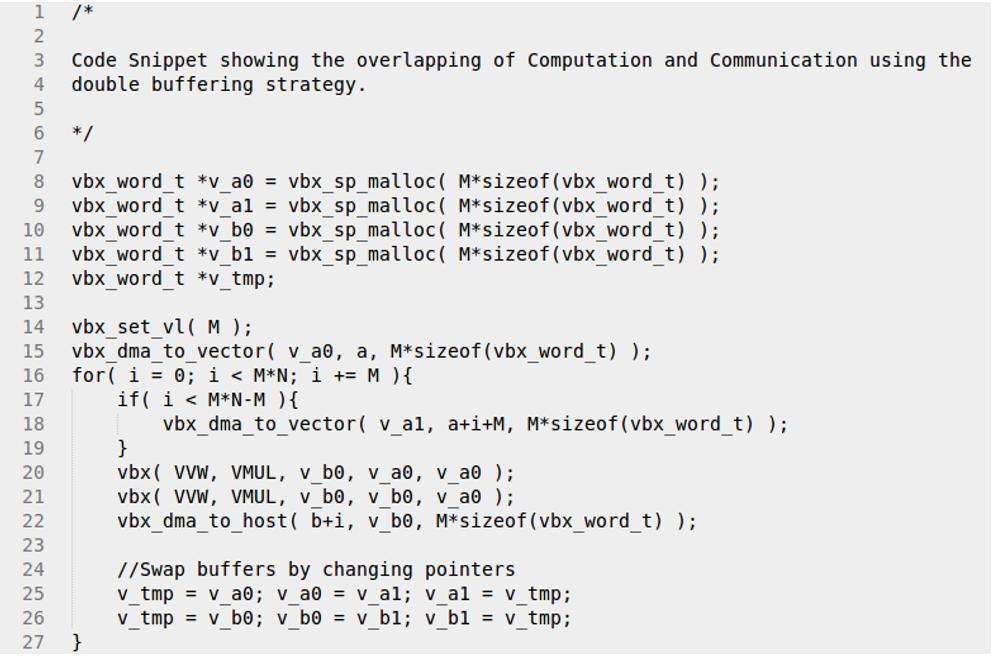
\includegraphics[width=0.9\textwidth]{images/c2.png}
	\caption{Overlapping Computation with Communication}
	\label{c2:mat}
\end{figure}

Consider the code in figure~\ref{c2:mat} which shows the overlapping of the communication and computation.
The same concept is used in measuring the performance for huge set of input data samples in chapter 5.


\section{Programming Model}
A basic program for MXP can be written by following the procedure below:

\begin{enumerate}

	\item Allocate the vectors in local scratchpad.

	\item DMA transfer from DDR to the local scratchpad.

	\item Set the vector length register. It indicates the number of vector elements on which the vector operations are to be performed.

	\item Perform vector operations and obtain result.

	\item Move data from the scratchpad to DDR. DMA transfer of result from local scratchpad to the DDR.

\end{enumerate}

\begin{figure}
	\centering
	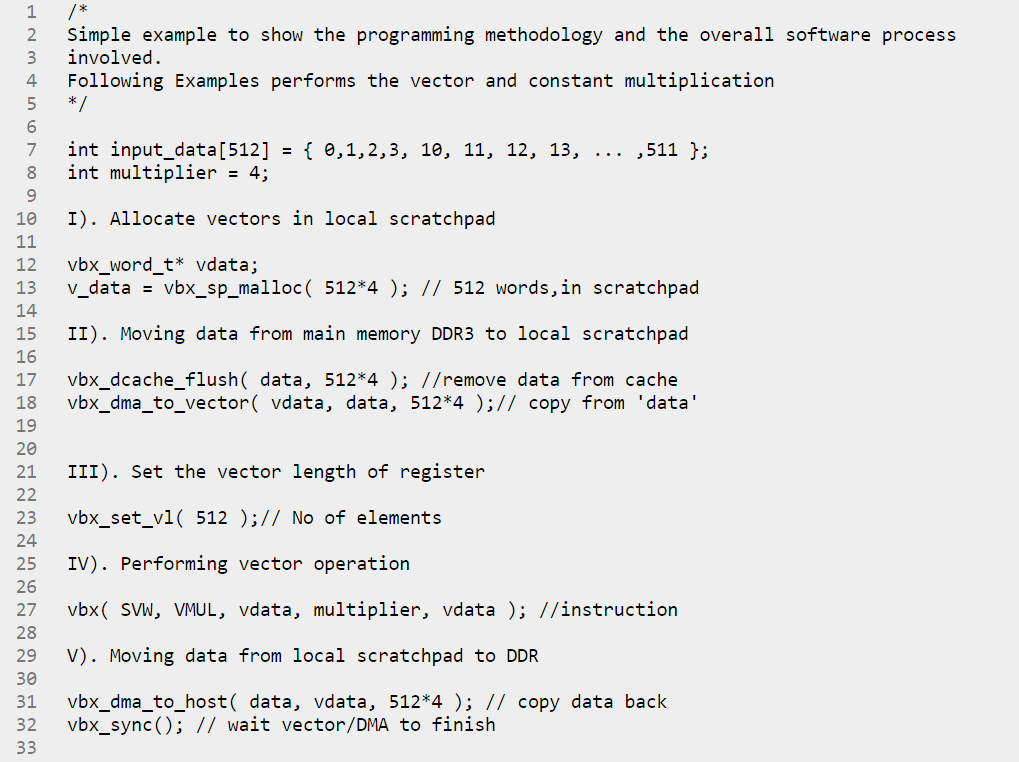
\includegraphics[width=.9\textwidth]{images/MXPProcess.png}
	\caption{Overall Software Process followed by MXP}
	\label{c3:mat}
\end{figure}



A sample example to explain the methodology is shown in Figure~\ref{c3:mat} The details of the programming methodology used can be found at \cite{20}. The figure shows a sample MXP program with the overall software process followed by MXP. The program shown in Figure~\ref{c3:mat} works fine in a bare-metal system. 

%\subsection{What if we want to run any image and audio processing application?}

In the case when we want to run any image and audio processing application, we will need a filesystem through which information in form of bytes from the input file can be extracted without having to manually enter values as in the example above. Also, the results after processing needs to be written to a file in the appropriate file format depending on the input file type. Vectorblox do provide sources for Linux containing necessary device drivers along with prebuilt bitstreams and hardware design file generated through Vivado.

We provide detailed steps for setting up Linux OS to use MXP on the ZedBoard so that it becomes easy for others to develop application and make full use of the system. Chapter 4 consist of the detailed information on how the Linux can be set up to use MXP.

